\documentclass[tikz,border=2pt]{standalone}
\usepackage{pgfplots}
\pgfplotsset{compat=1.18}
\begin{document}
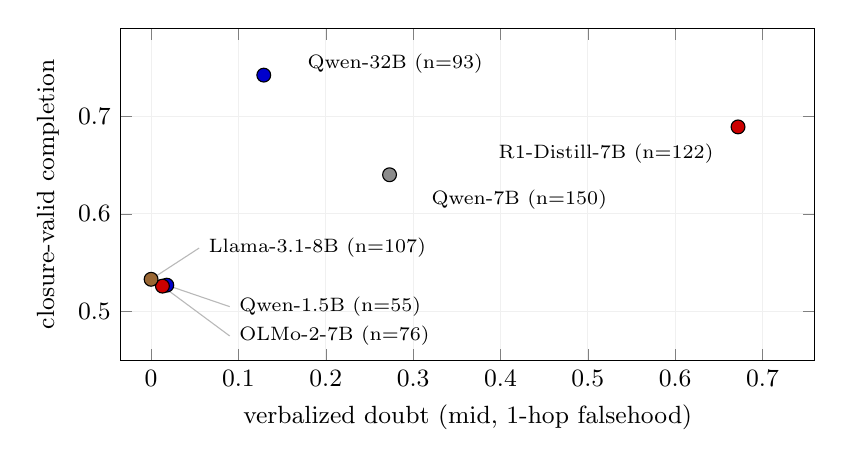
\begin{tikzpicture}
\begin{axis}[
  width=10.4cm,height=5.8cm,
  xmin=-.035,xmax=.76,ymin=.45,ymax=.79,
  xlabel={verbalized doubt (mid, 1-hop falsehood)},
  ylabel={closure-valid completion},
  grid=both,grid style={gray!12},
  tick label style={font=\small},label style={font=\small},
  clip=false,
]
\addplot+[only marks,mark=*,mark size=2.5pt,draw=black,fill=gray] coordinates {(0.018,0.527)};
\addplot+[only marks,mark=*,mark size=2.5pt,draw=black,fill=green!55!black] coordinates {(0.013,0.526)};
\addplot+[only marks,mark=*,mark size=2.5pt,draw=black,fill=olive] coordinates {(0.000,0.533)};
\addplot+[only marks,mark=*,mark size=2.5pt,draw=black,fill=black!45] coordinates {(0.273,0.640)};
\addplot+[only marks,mark=*,mark size=2.5pt,draw=black,fill=cyan!70!black] coordinates {(0.129,0.742)};
\addplot+[only marks,mark=*,mark size=2.5pt,draw=black,fill=red!70!black] coordinates {(0.672,0.689)};
\draw[gray!55,thin] (axis cs:0.018,0.527) -- (axis cs:0.090,0.505);
\draw[gray!55,thin] (axis cs:0.013,0.526) -- (axis cs:0.090,0.475);
\draw[gray!55,thin] (axis cs:0.000,0.533) -- (axis cs:0.055,0.565);
\node[anchor=west,font=\scriptsize] at (axis cs:0.090,0.505) {Qwen-1.5B (n=55)};
\node[anchor=west,font=\scriptsize] at (axis cs:0.090,0.475) {OLMo-2-7B (n=76)};
\node[anchor=west,font=\scriptsize] at (axis cs:0.055,0.565) {Llama-3.1-8B (n=107)};
\node[anchor=west,font=\scriptsize] at (axis cs:0.310,0.615) {Qwen-7B (n=150)};
\node[anchor=west,font=\scriptsize] at (axis cs:0.168,0.754) {Qwen-32B (n=93)};
\node[anchor=east,font=\scriptsize] at (axis cs:0.655,0.662) {R1-Distill-7B (n=122)};
\end{axis}
\end{tikzpicture}
\end{document}
